%----------------------------------------------------------------------------------------
% COVARIANTIE EN CORRELATIE. Alle opgaven zijn eigen werk; alle gegevens zijn verzonnen.
%
% Opbouw: Probleem, Start, leerstof (theorie, werkwijze of uitleg, voorbeeld, korte oefening), en op een
% nieuwe pagina de Opdrachten (door elkaar, stijgende moeilijkheid), Koppel en Test jezelf.
% Labels van dit hoofdstuk beginnen met h1-.
%----------------------------------------------------------------------------------------

\mychapter{1}{Covariantie en correlatie}

\begin{probleem}
\naast{Zes volwassenen noteren hoeveel uur ze per week sporten ($x$) en meten hun hartslag in rust ($y$, in slagen per minuut).

\smallskip
\kleinetabel[$x$ (uur)][$y$ (sl/min)]{6}{0 & 2 & 3 & 5 & 6 & 8}{74 & 70 & 68 & 63 & 64 & 57}

\smallskip
Sara wil met één getal zeggen hoe sterk $x$ en $y$ samen variëren. Ze vermenigvuldigt bij elke persoon de afwijkingen tot het gemiddelde, $(x_i - \xbar)(y_i - \ybar)$, en neemt het gemiddelde (gedeeld door $n - 1$): ze vindt $-17$. Bram doet hetzelfde, maar met de sporttijd in minuten, en vindt $-1020$. Hangen de gegevens van Bram sterker samen? Is $-17$ veel of weinig? En hoe groot kan zo'n getal worden?}{\begin{tikzpicture}[x=.5cm,y=.2cm,font=\scriptsize]
  \diagram[$x$ (uur)][$y$ (sl/min)]{0}{1}{9}{54}{2}{76}
  \xas{0,2,...,8}\yas{54,60,...,72}
  \punten[inkt]{(0,74) (2,70) (3,68) (5,63) (6,64) (8,57)}
\end{tikzpicture}}
\end{probleem}

\lkr{Leerplan Complementair (III-WiCo-d): LPD 54 (de correlatiecoëfficiënt als maat voor de samenhang hanteren), met de wenken: de formele definitie en het verband met de covariantie, het bewijs van $0 \leqslant r^2 \leqslant 1$ met de ongelijkheid van Cauchy-Schwarz, en de link met $R^2$ uit Lineaire regressie. De covariantie van twee variabelen bereidt LPD 53 voor (de covariantiematrix, hoofdstuk 2). Voorkennis uit pakket 4: Statistiek (gemiddelde en standaardafwijking met $n - 1$, hoofdstuk 1 over samenhang en causaliteit), Ruimtemeetkunde (het scalair product en de hoek tussen twee vectoren), en uit de 2de graad het spreidingsdiagram en $r$ met ICT. Wie Lineaire regressie zag, kent $\Sxx$, $\Sxy$, $\Syy$ en $R^2 = r^2$; het hoofdstuk verwijst ernaar, maar steunt er niet op. Extra: $r$ als cosinus van een hoek, het geval $r = \pm 1$, en de beperkingen van $r$ met samengevoegde groepen. Op de TI-84 geeft \texttt{LinReg(ax+b)} (met \texttt{DiagnosticOn}) $r$, en \texttt{2-Var Stats} de sommen $\sum xy$, $s_x$ en $s_y$; de covariantie zelf geeft het toestel niet. In een rekenblad: \texttt{COVARIANCE.S} en \texttt{CORREL} (in het Nederlands \texttt{COVARIANTIE.S} en \texttt{CORRELATIE}): controleer de namen in het programma van de school.}

In de 2de graad zag je in een spreidingsdiagram of twee variabelen samenhangen, en liet je ICT de correlatiecoëfficiënt $r$ berekenen. Waar die formule vandaan komt, en waarom $r$ altijd tussen $-1$ en $1$ ligt, bleef open. In dit hoofdstuk bouw je $r$ op uit een eenvoudiger getal: de \textit{covariantie}, die meet hoe twee variabelen samen variëren. Je ziet waarom de covariantie afhangt van de eenheden en $r$ niet, en je bewijst met de ongelijkheid van Cauchy-Schwarz dat $r^2 \leqslant 1$. Tot slot zie je wat $r$ niet zegt. Op het einde beantwoord je de vragen van Sara en Bram.

\begin{oefeningen}[Start]
\oef{h1-start-1}

\needspace{12\baselineskip}
\oef{h1-verken}
\end{oefeningen}

\lkr{De Verken laat de leerlingen zelf zien dat het teken van $(x_i - \xbar)(y_i - \ybar)$ afhangt van het kwadrant rond het gemiddelde punt. Laat ze de rechthoeken echt tekenen: de figuur in sectie 1 doet hetzelfde.}

%========================================================================================
\section{Samen variëren}

\subsection{De covariantie}

Hoe meet je of twee variabelen samen stijgen? Teken door het gemiddelde punt $(\xbar, \ybar)$ een horizontale en een verticale lijn. Ligt een punt rechtsboven of linksonder, dan liggen $x_i$ en $y_i$ allebei boven of allebei onder hun gemiddelde: het product $(x_i - \xbar)(y_i - \ybar)$ is positief. Ligt een punt linksboven of rechtsonder, dan is het product negatief. Tel je alle producten op, dan weet je welke kant de overhand heeft.

\naast{\begin{minipage}{9.4cm}
Het product heeft ook een meetkundige betekenis: het is de oppervlakte van de rechthoek met als hoekpunten het gemiddelde punt en het punt $(x_i, y_i)$, met een plus- of minteken. In de figuur zijn de positieve rechthoeken fel, de negatieve grijs. Zijn de felle samen groter, dan stijgt de wolk. De som is $\Sxy$ uit Lineaire regressie. Delen door $n - 1$ geeft een soort gemiddelde, zoals bij de variantie. Waarom $n - 1$ en niet $n$? Om dezelfde reden als bij de standaardafwijking in Statistiek: de afwijkingen worden gemeten tot het gemiddelde van de steekproef zelf, en zijn daardoor iets te klein.
\end{minipage}}{\begin{tikzpicture}[x=.68cm,y=.68cm,font=\scriptsize]
  \diagram{0}{1}{7}{2}{1}{8}
  \xas{0,1,...,7}\yas{2,3,...,8}
  \fill[fel,fill opacity=.35,draw=fel!70!black] (4,5) rectangle (1,3);
  \fill[fel,fill opacity=.35,draw=fel!70!black] (4,5) rectangle (6,7);
  \fill[grijs,fill opacity=.3,draw=grijs] (4,5) rectangle (3,6);
  \gemlijnen{4}{5}{0}{7}{2}{8}
  \punten[inkt]{(1,3) (3,6) (4,4) (6,5) (6,7)}
  \gempunt{4}{5}
  \node[fel!70!black,font=\footnotesize] at (6.6,7.6) {$+$};
  \node[fel!70!black,font=\footnotesize] at (0.5,2.5) {$+$};
  \node[grijs,font=\footnotesize] at (0.5,7.6) {$-$};
  \node[grijs,font=\footnotesize] at (6.6,2.5) {$-$};
\end{tikzpicture}}

\begin{theorie}
De \textbf{\textcolor{accent}{covariantie}} van $n$ paren $(x_1, y_1), \ldots, (x_n, y_n)$ is

\vspace{1mm}
\qquad $\formule{s_{xy} = \frac{1}{n - 1}\som (x_i - \xbar)(y_i - \ybar)}$
\end{theorie}

Is $s_{xy} > 0$, dan stijgt de wolk: grote $x$ gaan meestal samen met grote $y$. Is $s_{xy} < 0$, dan daalt ze. Bij $s_{xy} \approx 0$ is er geen stijgende of dalende tendens. De drie figuren tonen het.

\figuren{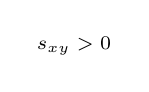
\begin{tikzpicture}[x=.36cm,y=.36cm,font=\scriptsize]
  \diagram{0}{1}{9}{0}{1}{9}
  \punten[inkt]{(1,2) (2,1.5) (2.5,3.5) (3.5,3) (4,4.5) (5,4) (5.5,6) (6.5,5.5) (7,7) (8,7.5)}
  \gemlijnen{4.5}{4.45}{0}{9}{0}{9}
  \node[below] at (4.5,-.6) {$s_{xy} > 0$};
\end{tikzpicture}\qquad
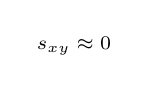
\begin{tikzpicture}[x=.36cm,y=.36cm,font=\scriptsize]
  \diagram{0}{1}{9}{0}{1}{9}
  \punten[inkt]{(1,5) (2,2) (2.5,7) (3.5,4) (4,8) (5,2.5) (5.5,5.5) (6.5,7.5) (7,3) (8,5.5)}
  \gemlijnen{4.5}{5}{0}{9}{0}{9}
  \node[below] at (4.5,-.6) {$s_{xy} \approx 0$};
\end{tikzpicture}\qquad
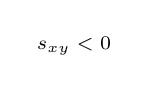
\begin{tikzpicture}[x=.36cm,y=.36cm,font=\scriptsize]
  \diagram{0}{1}{9}{0}{1}{9}
  \punten[inkt]{(1,8) (2,7.5) (2.5,6) (3.5,6.5) (4,5) (5,5.5) (5.5,3.5) (6.5,4) (7,2.5) (8,1.5)}
  \gemlijnen{4.5}{5}{0}{9}{0}{9}
  \node[below] at (4.5,-.6) {$s_{xy} < 0$};
\end{tikzpicture}}

\voorbeeld{}{Bereken de covariantie van de punten $(1, 3)$, $(3, 6)$, $(4, 4)$, $(6, 5)$ en $(6, 7)$ uit de figuur met de rechthoeken.\label{vb:h1-cov}}{%
\uitleg{De gemiddelden zijn gehele getallen, dus rekenen we met de afwijkingen: per punt het product, dan de som, en die delen we door $n - 1 = 4$.}
\begin{stappenbreed}
\xbar = \tfrac{20}{5} = 4, \quad \ybar = \tfrac{25}{5} = 5 & Het gemiddelde punt. \\[1ex]
x_i - \xbar\colon\ {-3},\ {-1},\ 0,\ 2,\ 2 \qquad y_i - \ybar\colon\ {-2},\ 1,\ {-1},\ 0,\ 2 & De afwijkingen. \\[1ex]
\text{producten}\colon\ 6,\ {-1},\ 0,\ 0,\ 4 \quad\text{som } 9 & De rechthoeken uit de figuur. \\[1ex]
s_{xy} = \tfrac{9}{4} = 2{,}25 & Delen door $n - 1$.
\end{stappenbreed}
De covariantie is positief: de wolk stijgt. Het punt $(3, 6)$ ligt linksboven en telt negatief mee, de twee punten op een gemiddelde lijn tellen niet mee.}

\begin{werkwijze}
Bereken $\xbar$ en $\ybar$. Zet in een tabel per paar de afwijkingen $x_i - \xbar$ en $y_i - \ybar$ en hun product. Tel de producten op en deel door $n - 1$. Kijk naar het teken: past het bij de richting van de wolk?
\end{werkwijze}

\begin{oefeningen}
\oef{h1-cov}
\end{oefeningen}

\subsection{Een rekenformule}

Zijn de gemiddelden geen mooie getallen, dan is rekenen met de afwijkingen omslachtig. Net zoals bij de variantie kun je de som herschrijven met $\sum x_i y_i$, een som die het rekentoestel geeft.

\begin{theorie}
\begin{stelling}{Rekenformule voor de covariantie}
\qquad $\formule{s_{xy} = \frac{1}{n - 1}\Bigl(\som x_i y_i - n\,\xbar\,\ybar\Bigr)}$
\end{stelling}

\begin{bewijs}
Werk het product uit en splits de som:
\bewijsregel{\som (x_i - \xbar)(y_i - \ybar) = \som x_i y_i - \ybar\som x_i - \xbar\som y_i + n\,\xbar\,\ybar .}
Omdat $\som x_i = n\xbar$ en $\som y_i = n\ybar$, zijn de tweede en de derde term allebei $-n\,\xbar\,\ybar$, zodat
\bewijsregel{\som (x_i - \xbar)(y_i - \ybar) = \som x_i y_i - 2n\,\xbar\,\ybar + n\,\xbar\,\ybar = \som x_i y_i - n\,\xbar\,\ybar .}
\end{bewijs}
\end{theorie}

\voorbeeld{}{Bereken de covariantie van $(1, 2)$, $(2, 5)$, $(4, 6)$ en $(6, 9)$.\label{vb:h1-rekenformule}}{%
\uitleg{De gemiddelden $3{,}25$ en $5{,}5$ zijn geen gehele getallen. Met de rekenformule hebben we alleen $\sum x_i y_i$ nodig.}
\begin{stappenbreed}
\xbar = 3{,}25, \quad \ybar = 5{,}5 & De gemiddelden. \\[1ex]
\som x_i y_i = 2 + 10 + 24 + 54 = 90 & De som van de producten. \\[1ex]
s_{xy} = \tfrac{1}{3}\bigl(90 - 4 \cdot 3{,}25 \cdot 5{,}5\bigr) = \tfrac{18{,}5}{3} \approx 6{,}17 & Met $n = 4$.
\end{stappenbreed}
Rond pas op het einde af: in $\sum x_i y_i - n\,\xbar\,\ybar$ trek je twee grote, bijna gelijke getallen van elkaar af, en een afronding in $\xbar$ telt daar zwaar door.}

\begin{oefeningen}
\oef{h1-rekenformule}
\end{oefeningen}

\subsection{Covariantie en variantie}

Wat is de covariantie van een variabele met zichzelf? Vervang je overal $y$ door $x$, dan staat er de formule van de variantie.

\begin{theorie}
\begin{stelling}{Covariantie met zichzelf}
\qquad $\formule{s_{xx} = s_x^2}$ \qquad en \qquad $\formule{s_{yx} = s_{xy}}$
\end{stelling}
\end{theorie}

Dat volgt meteen uit de definitie: $(x_i - \xbar)(x_i - \xbar) = (x_i - \xbar)^2$, en een product van twee getallen verandert niet als je ze omwisselt. Een bewijs in een kader is overbodig. De covariantie is dus een veralgemening van de variantie: de variantie meet hoe één variabele varieert, de covariantie hoe twee variabelen \textit{samen} variëren. In hoofdstuk 2 zetten we ze allemaal samen in één matrix.

\subsection{Andere eenheden}

Wat gebeurt er met de covariantie als je een variabele in een andere eenheid uitdrukt? Meet je een tijd in minuten in plaats van in uren, dan worden alle $x$-waarden 60 keer zo groot. En wat als je een constante optelt, zoals bij een omzetting van graden Celsius naar Fahrenheit?

\begin{theorie}
\begin{stelling}{Covariantie en lineaire transformaties}
Als $u_i = a x_i + b$ en $v_i = c y_i + d$ voor alle $i$, dan is

\qquad $\formule{s_{uv} = ac \, s_{xy}}$
\end{stelling}

\begin{bewijs}
Het gemiddelde van de $u_i$ is $\overline u = a\xbar + b$, dus $u_i - \overline u = a(x_i - \xbar)$: de constante $b$ valt weg. Net zo is $v_i - \overline v = c(y_i - \ybar)$. Dan is
\bewijsregel{s_{uv} = \frac{1}{n - 1}\som a(x_i - \xbar) \cdot c(y_i - \ybar) = ac \, s_{xy} .}
\end{bewijs}
\end{theorie}

Een verschuiving verandert de covariantie dus niet, maar een andere schaal wel: de covariantie heeft als eenheid het product van de eenheden van $x$ en $y$. Daarom zegt een covariantie op zich weinig: bij een lengte in cm en een massa in kg is haar eenheid \textit{cm maal kg}. Uit de stelling volgt ook $s_{ax+b}^2 = s_{(ax+b)(ax+b)} = a^2 s_x^2$, wat je kent uit Statistiek.

\voorbeeld{}{Een ijsjesverkoper noteert op zes dagen de maximumtemperatuur $x$ (in °C) en het aantal verkochte ijsjes $y$. De covariantie is $s_{xy} = 244$. Hoe groot is de covariantie als de temperatuur in graden Fahrenheit staat? Een temperatuur van $x$~°C is $1{,}8x + 32$~°F.\label{vb:h1-eenheden}}{%
\uitleg{De temperatuur ondergaat een lineaire transformatie met $a = 1{,}8$ en $b = 32$; het aantal ijsjes blijft ($c = 1$, $d = 0$).}
\begin{stappenbreed}
s_{uv} = 1{,}8 \cdot 1 \cdot 244 = 439{,}2 & De verschuiving met 32 speelt geen rol.
\end{stappenbreed}
Dezelfde zes dagen geven een andere covariantie, alleen omdat een graad Fahrenheit kleiner is dan een graad Celsius. Het verband zelf is niet sterker geworden.}

\begin{oefeningen}
\oef{h1-eenheden}
\end{oefeningen}

%========================================================================================
\section{De correlatiecoëfficiënt}

\subsection{Een maat zonder eenheid}

De covariantie zegt welke richting de wolk heeft, maar niet hoe sterk de samenhang is: het getal hangt af van de eenheden. Hoe maak je er een maat van die dat niet doet? Deel door iets met dezelfde eenheid. De standaardafwijking $s_x$ heeft de eenheid van $x$ en $s_y$ die van $y$: deel dus door hun product.

\begin{theorie}
De \textbf{\textcolor{accent}{correlatiecoëfficiënt}} van $n$ paren $(x_i, y_i)$, met $s_x > 0$ en $s_y > 0$, is

\vspace{1mm}
\qquad $\formule{r = \frac{s_{xy}}{s_x\,s_y}}$
\end{theorie}

Schrijf je alles uit, dan vallen de factoren $\frac{1}{n - 1}$ weg, en krijg je de formule uit de 2de graad en uit Lineaire regressie:
\[ r = \frac{\frac{1}{n-1}\Sxy}{\sqrt{\frac{1}{n-1}\Sxx}\,\sqrt{\frac{1}{n-1}\Syy}} = \frac{\Sxy}{\sqrt{\Sxx\,\Syy}} \qquad\text{met}\quad \Sxy = \som (x_i - \xbar)(y_i - \ybar) . \]
Het maakt voor $r$ dus niet uit of je door $n$ of door $n - 1$ deelt. Is $s_x = 0$, dan zijn alle $x_i$ gelijk en liggen alle punten op een verticale rechte: dan bestaat $r$ niet.

\begin{theorie}
\begin{stelling}{Correlatie en lineaire transformaties}
Als $u_i = a x_i + b$ en $v_i = c y_i + d$ met $a, c \neq 0$, dan is

\qquad $\formule{r_{uv} = r_{xy}}$ \ als $ac > 0$ \qquad en \qquad $\formule{r_{uv} = -r_{xy}}$ \ als $ac < 0$
\end{stelling}

\begin{bewijs}
Uit de vorige stelling is $s_{uv} = ac\,s_{xy}$, $s_u^2 = a^2 s_x^2$ en $s_v^2 = c^2 s_y^2$, dus $s_u = \abs{a}\,s_x$ en $s_v = \abs{c}\,s_y$. Dan is
\bewijsregel{r_{uv} = \frac{ac\,s_{xy}}{\abs{a}\,s_x\,\abs{c}\,s_y} = \frac{ac}{\abs{ac}}\,r_{xy} ,}
en $\frac{ac}{\abs{ac}}$ is $1$ als $ac > 0$ en $-1$ als $ac < 0$.
\end{bewijs}
\end{theorie}

Andere eenheden of een ander nulpunt veranderen $r$ dus niet. Alleen het teken kan omslaan, als je één van de variabelen omkeert: de score op een toets en het aantal \textit{fouten} hebben een tegengestelde correlatie met de studietijd.

\voorbeeld{}{Bereken de correlatiecoëfficiënt van de punten $(1, 3)$, $(3, 6)$, $(4, 4)$, $(6, 5)$ en $(6, 7)$ uit voorbeeld \ref{vb:h1-cov}.\label{vb:h1-r}}{%
\uitleg{De covariantie $s_{xy} = 2{,}25$ kennen we al. We berekenen de twee varianties met dezelfde afwijkingen.}
\begin{stappenbreed}
s_x^2 = \tfrac{9 + 1 + 0 + 4 + 4}{4} = 4{,}5, \quad s_y^2 = \tfrac{4 + 1 + 1 + 0 + 4}{4} = 2{,}5 & De kwadraten van de afwijkingen. \\[1ex]
r = \frac{2{,}25}{\sqrt{4{,}5}\,\sqrt{2{,}5}} = \frac{2{,}25}{\sqrt{11{,}25}} \approx 0{,}671 & De definitie.
\end{stappenbreed}
Een matige positieve samenhang. \texttt{LinReg(ax+b)} geeft hetzelfde getal.}

\begin{oefeningen}
\oef{h1-r}
\end{oefeningen}

%========================================================================================
\section{Waarom ligt $r$ tussen $-1$ en $1$?}

\subsection{Twee vectoren}

In de 2de graad zag je dat $r$ tussen $-1$ en $1$ ligt. Waarom kan $\abs{s_{xy}}$ nooit groter zijn dan $s_x s_y$? Kijk naar de afwijkingen als twee vectoren met $n$ componenten:
\[ \vec u = (x_1 - \xbar,\ x_2 - \xbar,\ \ldots,\ x_n - \xbar) \qquad\text{en}\qquad \vec v = (y_1 - \ybar,\ y_2 - \ybar,\ \ldots,\ y_n - \ybar) . \]
Bij $n = 3$ zijn dat gewone vectoren in de ruimte. Dan is $\Sxy = \vec u \cdot \vec v$ hun scalair product, en zijn $\Sxx = \abs{\vec u}^2$ en $\Syy = \abs{\vec v}^2$ de kwadraten van hun normen. De correlatiecoëfficiënt wordt
\[ r = \frac{\vec u \cdot \vec v}{\abs{\vec u}\,\abs{\vec v}} , \]
en uit Ruimtemeetkunde ken je dat quotiënt: het is de cosinus van de hoek tussen $\vec u$ en $\vec v$. Een cosinus ligt altijd tussen $-1$ en $1$. Maar meestal is $n$ groter dan 3. Wat is een hoek tussen twee vectoren met tien componenten? Daarvoor hebben we eerst een ongelijkheid nodig die zegt dat het quotiënt ook dan tussen $-1$ en $1$ ligt.

\subsection{De ongelijkheid van Cauchy-Schwarz}

Het idee van het bewijs: een som van kwadraten is nooit negatief. Neem een getal $t$ en bekijk $\som (t u_i + v_i)^2$. Die som is een tweedegraadsfunctie van $t$ die nooit negatief wordt, en dat legt haar discriminant vast.

\begin{theorie}
\begin{stelling}{Ongelijkheid van Cauchy-Schwarz}
Voor alle reële getallen $u_1, \ldots, u_n$ en $v_1, \ldots, v_n$ is

\qquad $\formule{\Bigl(\som u_i v_i\Bigr)^2 \leqslant \som u_i^2 \cdot \som v_i^2}$

Er geldt een gelijkheid als en slechts als alle $u_i = 0$, of er een $t$ is met $v_i = -t\,u_i$ voor alle $i$.
\end{stelling}

\begin{bewijs}
Stel $A = \som u_i^2$, $B = \som u_i v_i$ en $C = \som v_i^2$. Zijn alle $u_i = 0$, dan zijn beide leden 0. Neem dus $A > 0$. Voor elke $t \in \R$ is
\bewijsregel{f(t) = \som (t u_i + v_i)^2 = A t^2 + 2B t + C \geqslant 0 .}
Een tweedegraadsfunctie met $A > 0$ die nergens negatief is, heeft hoogstens één nulwaarde, dus haar discriminant is niet positief:
\bewijsregel{4B^2 - 4AC \leqslant 0 , \quad\text{dus}\quad B^2 \leqslant AC .}
Een gelijkheid $B^2 = AC$ betekent discriminant 0: dan is er een $t$ met $f(t) = 0$. Een som van kwadraten is 0 als en slechts als elk kwadraat 0 is, dus $t u_i + v_i = 0$ voor alle $i$. Omgekeerd geeft $v_i = -t u_i$ meteen $B^2 = t^2 A^2 = AC$.
\end{bewijs}
\end{theorie}

\naast{\begin{minipage}{10cm}
De figuur toont het idee: de parabool $f(t) = At^2 + 2Bt + C$ ligt helemaal boven de horizontale as, of raakt ze in één punt. Ze kan de as niet snijden, want dan zou $f$ tussen de twee nulwaarden negatief zijn. In woorden zegt de ongelijkheid: het scalair product van twee vectoren is in absolute waarde hoogstens het product van hun normen, $\abs{\vec u \cdot \vec v} \leqslant \abs{\vec u}\,\abs{\vec v}$, en dat in elke dimensie. De Franse wiskundige Augustin-Louis Cauchy bewees ze in 1821 voor sommen; Hermann Schwarz bewees in 1888 de versie voor integralen.
\end{minipage}}{\begin{tikzpicture}[x=.55cm,y=.3cm,font=\scriptsize]
  \draw[->,grijs] (-4,0) -- (2.2,0) node[right,text=black] {$t$};
  \draw[->,grijs] (0,-.8) -- (0,8.5) node[above,text=black] {$f(t)$};
  \kromme{-3.6}{1.4}{0.8*(\x+1.1)^2+1.2}
  \kromme[tweede]{-3.4}{1.6}{0.8*(\x+0.9)^2}
  \node[accent,left] at (-3.6,7.4) {$D < 0$};
  \node[inkt,below] at (-0.9,0) {$D = 0$};
\end{tikzpicture}}

\voorbeeld{}{Controleer de ongelijkheid van Cauchy-Schwarz voor $\vec u = (1, 2, 3)$ en $\vec v = (2, -1, 4)$, en voor $\vec u = (1, -2, 2)$ en $\vec v = (-3, 6, -6)$.\label{vb:h1-cs}}{%
\uitleg{We berekenen telkens het scalair product en de twee kwadratensommen. Bij het tweede paar valt op dat $\vec v = -3\vec u$.}
\begin{stappenbreed}
(2 - 2 + 12)^2 = 144 \leqslant (1 + 4 + 9)(4 + 1 + 16) = 294 & Het eerste paar: strikt kleiner. \\[1ex]
(-3 - 12 - 12)^2 = 729 = (1 + 4 + 4)(9 + 36 + 36) = 729 & Het tweede paar: gelijk.
\end{stappenbreed}
Bij het tweede paar is $\vec v = -t\vec u$ met $t = 3$: de vectoren liggen op één rechte, en dan geldt de gelijkheid.}

\begin{oefeningen}
\oef{h1-cs}
\end{oefeningen}

\subsection{De gevolgen voor $r$}

Pas de ongelijkheid toe op de afwijkingen $u_i = x_i - \xbar$ en $v_i = y_i - \ybar$. Dan staat er $\Sxy^2 \leqslant \Sxx\,\Syy$, en dat is precies wat we zochten.

\begin{theorie}
\begin{stelling}{Grenzen van de correlatiecoëfficiënt}
\qquad $\formule{0 \leqslant r^2 \leqslant 1}$ \qquad dus \qquad $\formule{-1 \leqslant r \leqslant 1}$
\end{stelling}

\begin{bewijs}
Met $u_i = x_i - \xbar$ en $v_i = y_i - \ybar$ geeft Cauchy-Schwarz $\Sxy^2 \leqslant \Sxx\,\Syy$. Omdat $s_x, s_y > 0$, is $\Sxx\,\Syy > 0$, en
\bewijsregel{r^2 = \frac{\Sxy^2}{\Sxx\,\Syy} \leqslant 1 .}
Een kwadraat is nooit negatief, dus $0 \leqslant r^2$.
\end{bewijs}

\begin{stelling}{Perfecte correlatie}
$\formule{r = 1}$ of $\formule{r = -1}$ als en slechts als alle punten op één rechte $y = mx + q$ met $m \neq 0$ liggen. Het teken van $r$ is dat van $m$.
\end{stelling}

\begin{bewijs}
$r^2 = 1$ betekent een gelijkheid in Cauchy-Schwarz. Omdat niet alle $u_i$ nul zijn ($s_x > 0$), bestaat er een $t$ met $y_i - \ybar = -t(x_i - \xbar)$ voor alle $i$: alle punten liggen op de rechte door $(\xbar, \ybar)$ met richtingscoëfficiënt $m = -t$, en $m \neq 0$ omdat $s_y > 0$. Omgekeerd: liggen de punten op $y = mx + q$, dan is $v_i = m u_i$, en
\bewijsregel{r = \frac{\som u_i \cdot m u_i}{\sqrt{\som u_i^2}\,\sqrt{m^2 \som u_i^2}} = \frac{m}{\abs{m}} = \pm 1 .}
\end{bewijs}
\end{theorie}

Nu kunnen we ook in elke dimensie een hoek definiëren: omdat het quotiënt tussen $-1$ en $1$ ligt, is er één hoek $\theta \in [0^\circ, 180^\circ]$ met $\cos\theta = r$. De correlatiecoëfficiënt is de cosinus van de hoek tussen de vectoren van de afwijkingen. Bij $r = 1$ wijzen ze in dezelfde richting, bij $r = 0$ staan ze loodrecht op elkaar, bij $r = -1$ wijzen ze tegengesteld. Wie Lineaire regressie zag, kent nog een bewijs van $r^2 \leqslant 1$: daar is $r^2$ de determinatiecoëfficiënt $R^2$, het deel van de variatie in $y$ dat de regressierechte verklaart, en dat deel is hoogstens 1.

\voorbeeld{}{Bereken de correlatiecoëfficiënt van $(1, 2)$, $(2, 5)$ en $(3, 5)$ als de cosinus van een hoek. Hoe groot is die hoek?\label{vb:h1-hoek}}{%
\uitleg{Met drie punten zijn de vectoren van de afwijkingen gewone vectoren in de ruimte.}
\begin{stappenbreed}
\vec u = (-1, 0, 1), \quad \vec v = (-2, 1, 1) & Met $\xbar = 2$ en $\ybar = 4$. \\[1ex]
r = \frac{2 + 0 + 1}{\sqrt{2}\,\sqrt{6}} = \frac{3}{\sqrt{12}} = \frac{\sqrt3}{2} \approx 0{,}866 & Scalair product gedeeld door de normen. \\[1ex]
\theta = 30^\circ & Want $\cos 30^\circ = \frac{\sqrt3}{2}$.
\end{stappenbreed}
De vectoren van de afwijkingen maken een hoek van $30^\circ$. Hoe kleiner de hoek, hoe sterker de positieve samenhang.}

\begin{oefeningen}
\oef{h1-hoek}
\end{oefeningen}

\subsection{$r$ en de determinatiecoëfficiënt}

Hoe interpreteer je de grootte van $r$? Een tabel met grenzen, zoals \textit{sterk vanaf $0{,}8$}, is een afspraak, geen wiskunde. Beter is de link met Lineaire regressie: $r^2 = R^2$ is het deel van de variantie van $y$ dat de regressierechte verklaart. Een correlatie van $0{,}7$ klinkt sterk, maar verklaart maar $0{,}49$, minder dan de helft. Wie Lineaire regressie niet zag, kan het onthouden als: het kwadraat van $r$ zegt welk deel van de spreiding van $y$ samenhangt met $x$.

\begin{oefeningen}
\oef{h1-r2}
\end{oefeningen}

%========================================================================================
\section{Wat $r$ niet zegt}

\subsection{Alleen lineaire samenhang}

Een correlatie dicht bij 0 lijkt te zeggen dat er geen verband is. Klopt dat? De covariantie telt alleen of de punten rechtsboven en linksonder liggen, of linksboven en rechtsonder. Een verband dat eerst daalt en dan stijgt, valt daar niet onder.

\voorbeeld{}{Bereken de correlatiecoëfficiënt van de punten $(-2, 4)$, $(-1, 1)$, $(0, 0)$, $(1, 1)$ en $(2, 4)$.\label{vb:h1-parabool}}{%
\naast{\begin{minipage}{10cm}
\uitleg{De punten liggen symmetrisch rond de $y$-as. We berekenen de covariantie met de afwijkingen.}
\begin{stappenvrij}{5.6cm}{4.1cm}
\xbar = 0, \quad \ybar = 2 & Het gemiddelde punt. \\[1ex]
\text{producten}\colon\ {-4},\ 1,\ 0,\ {-1},\ 4 & $x_i(y_i - 2)$. \\[1ex]
s_{xy} = 0, \quad r = 0 & De som is 0.
\end{stappenvrij}
\end{minipage}}{\begin{tikzpicture}[x=.5cm,y=.45cm,font=\scriptsize]
  \draw[black!14,very thin] (-3,0) grid (3,5);
  \draw[->,grijs] (-3,0) -- (3.4,0) node[right,text=black] {$x$};
  \draw[->,grijs] (0,0) -- (0,5.4) node[above,text=black] {$y$};
  \kromme[accent!60]{-2.2}{2.2}{\x*\x}
  \draw[inkt,thin,dashed] (-3,2) -- (3,2);
  \punten[inkt]{(-2,4) (-1,1) (0,0) (1,1) (2,4)}
  \foreach \t in {-2,2}{\node[below] at (\t,0) {$\t$};}
  \node[left] at (0,4) {$4$};
\end{tikzpicture}}
De punten liggen precies op de parabool $y = x^2$: $y$ hangt volledig af van $x$. Toch is $r = 0$. Links compenseren de producten die rechts. De correlatiecoëfficiënt meet alleen \textit{lineaire} samenhang.}

Een covariantie van 0 betekent dus niet dat de variabelen niets met elkaar te maken hebben. Men zegt dan dat ze \textbf{ongecorreleerd} zijn, wat iets anders is dan onafhankelijk.

\subsection{Uitschieters}

De covariantie is een som van rechthoeken. Een punt ver van de rest geeft een enorme rechthoek, die de som kan domineren.

\voorbeeld{}{De punten $(1, 2)$, $(2, 1)$, $(3, 3)$, $(4, 2)$ en $(5, 2)$ hebben $r \approx 0{,}22$. Er komt één punt $(12, 10)$ bij. Bereken $r$ opnieuw met ICT.\label{vb:h1-uitschieter}}{%
\naast{\begin{minipage}{10cm}
\uitleg{We voegen het punt toe aan de lijsten en laten het rekentoestel $r$ berekenen. Daarna kijken we naar de rechthoek van het nieuwe punt.}
\begin{stappenvrij}{5.6cm}{4.1cm}
r \approx 0{,}932 & Met \texttt{LinReg(ax+b)}. \\[1ex]
(12 - 4{,}5)(10 - 3{,}33) = 50 & Het product van het nieuwe punt. \\[1ex]
\Sxy = 61 & De som van alle producten.
\end{stappenvrij}
\end{minipage}}{\begin{tikzpicture}[x=.3cm,y=.3cm,font=\scriptsize]
  \diagram{0}{2}{13}{0}{2}{11}
  \xas{0,4,...,12}\yas{0,4,8}
  \fill[fel,fill opacity=.3,draw=fel!70!black] (4.5,3.33) rectangle (12,10);
  \punten[inkt]{(1,2) (2,1) (3,3) (4,2) (5,2)}
  \punten[fel!80!black]{(12,10)}
  \gempunt{4.5}{3.33}
\end{tikzpicture}}
Eén punt maakt van een zwakke samenhang een schijnbaar sterke: het levert 50 van de 61 in $\Sxy$. Is het punt een meetfout, dan moet het weg. Is het echt, dan moet je het vermelden, en $r$ met en zonder dat punt geven.}

\subsection{Groepen, oorzaken en een beperkt bereik}

\naast{\begin{minipage}{11cm}
Ook zonder uitschieter kan $r$ misleiden. In de figuur rechts zijn er twee groepen van vijf punten. Binnen elke groep is $r = 0$, maar samen geven ze $r \approx 0{,}89$: het verschil tussen de groepen maakt de samenhang. Denk aan de schoenmaat en de score op een leestest bij kinderen van 6 en van 12 jaar. Het omgekeerde gebeurt bij een \textbf{beperkt bereik}: wie alleen leerlingen bekijkt die geslaagd zijn voor een toelatingsproef, vindt een zwakkere correlatie tussen die proef en de latere resultaten dan bij alle kandidaten. En zoals je in Statistiek zag: een sterke correlatie bewijst geen oorzaak. Een verborgen variabele (de leeftijd, bij de schoenmaat) kan beide variabelen sturen.
\end{minipage}}{\begin{tikzpicture}[x=.34cm,y=.34cm,font=\scriptsize]
  \diagram{0}{1}{9}{0}{1}{9}
  \xas{0,2,...,8}\yas{0,2,...,8}
  \punten[inkt]{(1,1) (1,3) (2,2) (3,1) (3,3)}
  \punten[fel!80!black]{(6,6) (6,8) (7,7) (8,6) (8,8)}
  \draw[grijs,dashed] (2,2) circle (1.8);
  \draw[grijs,dashed] (7,7) circle (1.8);
\end{tikzpicture}}

\begin{werkwijze}
Teken eerst het spreidingsdiagram. Bereken $r$ alleen als de wolk ongeveer langs een rechte ligt, en zeg er de richting en de sterkte bij (met $r^2$ als deel van de verklaarde variantie). Zoek uitschieters en groepen, en geef $r$ dan ook zonder dat punt of per groep. Besluit nooit uit $r$ alleen dat de ene variabele de andere veroorzaakt.
\end{werkwijze}

\begin{oefeningen}
\oef{h1-beperking}
\end{oefeningen}

%========================================================================================
\needspace{16\baselineskip}
\subsection{Terug naar het probleem}

\voorbeeld{}{Terug naar het probleem. Zes volwassenen noteren hoeveel uur ze per week sporten ($x$) en meten hun hartslag in rust ($y$, in slagen per minuut).

\smallskip
\kleinetabel[$x$ (uur)][$y$ (sl/min)]{6}{0 & 2 & 3 & 5 & 6 & 8}{74 & 70 & 68 & 63 & 64 & 57}

\smallskip
Sara wil met één getal zeggen hoe sterk $x$ en $y$ samen variëren. Ze berekent de covariantie en vindt $s_{xy} = -17$. Bram doet hetzelfde, maar met de sporttijd in minuten, en vindt $-1020$. Hangen de gegevens van Bram sterker samen? Is $-17$ veel of weinig? En hoe groot kan zo'n maat voor de samenhang worden?\label{vb:h1-terug}}{%
\uitleg{Bram vermenigvuldigt de $x$-waarden met 60. We berekenen de standaardafwijkingen en de correlatiecoëfficiënt voor beiden.}
\begin{stappenbreed}
-1020 = 60 \cdot (-17) & De covariantie wordt 60 keer zo groot ($a = 60$). \\[1ex]
\Sxx = 42, \quad \Syy = 178, \quad \Sxy = -85 & Met $\xbar = 4$ en $\ybar = 66$. \\[1ex]
r = \frac{-85}{\sqrt{42 \cdot 178}} \approx -0{,}983 & Voor Sara. \\[1ex]
s_x = 60 \cdot \sqrt{8{,}4} \approx 173{,}9 \colon\ r = \frac{-1020}{173{,}9 \cdot 5{,}967} \approx -0{,}983 & Voor Bram: dezelfde $r$. \\[1ex]
r^2 \approx 0{,}966 & Het verklaarde deel.
\end{stappenbreed}
De samenhang is bij beiden even sterk: het zijn dezelfde mensen, alleen in andere eenheden. De covariantie hangt af van de eenheden, de correlatiecoëfficiënt niet. Met $r \approx -0{,}98$ is de samenhang zeer sterk en dalend: wie meer sport, heeft een lagere rusthartslag, en de sporttijd verklaart ongeveer 97~\% van de variantie in de hartslag van deze zes mensen. Willekeurig groot wordt $r$ niet: door Cauchy-Schwarz is altijd $-1 \leqslant r \leqslant 1$. Dat sporten de oorzaak is, is aannemelijk, maar volgt niet uit zes metingen: wie gezonder is, sport misschien ook meer.}

%========================================================================================
\opdrachtenkop

\begin{oefeningen}
\oef{h1-o1}

\oef{h1-o2}

\needspace{10\baselineskip}
\oef{h1-o3}

\oef{h1-o4}

\needspace{10\baselineskip}
\oef{h1-o5}

\oef{h1-o6}

\needspace{12\baselineskip}
\oef{h1-o7}

\oef{h1-o8}

\needspace{12\baselineskip}
\oef{h1-o9}

\oef{h1-o10}

\needspace{12\baselineskip}
\oef{h1-o11}

\oef{h1-o12}

\needspace{12\baselineskip}
\oef{h1-o13}

\oef{h1-o14}

\needspace{12\baselineskip}
\oef{h1-o15}

\oef{h1-o16}

\needspace{12\baselineskip}
\oef{h1-o17}

\oef{h1-o18}

\needspace{12\baselineskip}
\oef{h1-o19}

\oef{h1-o20}

\needspace{12\baselineskip}
\oef{h1-o21}
\end{oefeningen}

%----------------------------------------------------------------------------------------
% KOPPEL: verbanden met andere leerstof
%----------------------------------------------------------------------------------------
\needspace{20\baselineskip}
\opdrachtsectie{Koppel}

\lkr{De eerste oefening steunt op het scalair product en de hoek tussen vectoren (Ruimtemeetkunde, hoofdstuk 4), de tweede op de regressierechte en $R^2$ (Lineaire regressie, hoofdstuk 1 en 2), de derde op de stelling van Pythagoras en de cosinusregel, en de vierde op Statistiek (hoofdstuk 1: samenhang en causaliteit).}

\begin{oefeningen}
\oef{h1-koppel-1}

\oef{h1-koppel-2}

\oef{h1-koppel-3}

\oef{h1-koppel-4}
\end{oefeningen}

%----------------------------------------------------------------------------------------
\opdrachtsectie{Test jezelf}

\begin{oefeningen}
\oef{h1-t1}

\oef{h1-t2}

\oef{h1-t3}

\oef{h1-t4}

\oef{h1-t5}

\oef{h1-t6}

\oef{h1-t7}
\end{oefeningen}

\herhaalschema{%
  \fv{oef:h1-t1}{vb:h1-cov}{oef:h1-cov}%
  \fv{oef:h1-t2}{vb:h1-rekenformule}{oef:h1-rekenformule}%
  \fv{oef:h1-t3}{vb:h1-eenheden}{oef:h1-eenheden}%
  \fv{oef:h1-t4}{vb:h1-r}{oef:h1-r}%
  \fv{oef:h1-t5}{vb:h1-cs}{oef:h1-cs}%
  \fv{oef:h1-t6}{vb:h1-hoek}{oef:h1-hoek}%
  \fv{oef:h1-t7}{vb:h1-parabool}{oef:h1-beperking}}

\ifzelfstudie
\section*{Maak je eigen samenvatting}
Sluit dit boek en schrijf in je schrift: de definitie van de covariantie met de betekenis van haar teken (de rechthoeken rond het gemiddelde punt), de rekenformule met het bewijs, het verband met de variantie, wat een lineaire transformatie met de covariantie doet, de definitie van $r$ en waarom $r$ niet van de eenheden afhangt, de vectoren van de afwijkingen, de ongelijkheid van Cauchy-Schwarz met het bewijs via de discriminant, waarom daaruit $-1 \leqslant r \leqslant 1$ volgt, wanneer $r = \pm 1$, $r$ als cosinus, de betekenis van $r^2$, en vier dingen die $r$ niet zegt. Vergelijk daarna met de kaders.
\fi
